\chapter{Existierende Auswahlkomponenten}
\label{chap:existingComponents}

Hier sind die Gegenüberstellungen der bereits vorhandenen Möglichkeiten zur Darstellung einer Optionsauswahl aufgelistet. 
Eine Auflistung der möglichen Funktionalitäten zeigt die Grenzen dieser Elemente auf. 
Dabei spielen die UI- als auch die Interaktions-Unterschiede dieser Komponenten in verschiedenen Browsern eine tragende Rolle. 

Als Basis dieser Arbeit dient das Country Select. 
Weiter existieren bereits die Elemente Buttons bzw. Links, \codestyle{select} und \codestyle{datalist}. 
Unter dem Country Select ist das Resultat der Vorarbeit zu verstehen. 
Die folgende Tabelle \ref{table:generalComparing} zeigt einen Vergleich der genannten Möglichkeiten. 

\import{../tables}{c.choice.general.tex}

Nebst den in der Tabelle aufgeführten Möglichkeiten existieren diverse Libraries und Frameworks. 
Viele dieser Lösungen für Auswahlkomponenten besitzen Abhängigkeiten zu weiteren Bibliothek-Komponenten. 
Durch das Einbinden der Frameworks bläst sich der eigene Code extrem auf. 
Diese Auswahlkomponenten bieten eine Menge an Funktionen an, welche jedoch die Anwendung sehr komplex machen. 
Die Einarbeitung dauert lange. 
Da das Ziel dieses Projekts eine schlanke und einfach verwendbare Komponente ist, sind die existierenden Frameworks keine Lösung. 
Dieser Bericht legt keinen weiteren Fokus auf externe Bibliotheken. 


\section{HTML Datalist vs. Select}
\label{sec:datalistSelect}

Die folgenden Unterkapitel zeigen die Möglichkeiten, welche die HTML-Elemente \codestyle{input}, \codestyle{option}, \codestyle{datalist} und \codestyle{select} bieten. 
Zudem zeigen tabellarische Gegenüberstellungen die Unterschiede und Inkonsistenzen dieser in verschiedenen Browsern und Betriebssystemen auf. 
Hierbei liegt der Fokus mehr auf der Interaktion mit den Komponenten als auf der Darstellung. 


\subsection{Option}
\label{sec:option}

Die beiden Auswahlkomponenten – \codestyle{datalist} und \codestyle{select} – verwenden \codestyle{option}-Elemente. 
Die einzelnen Optionen wie in Code \ref{code:optionExample} Zeile 1 besitzen ein \codestyle{value}-Attribut und einen Inhalt – das Label. 
Alternativ ist das \codestyle{label}-Attribut zu nutzen und dafür das Value an die Stelle des Inhalts zu platzieren. 
Firefox unterstützt diese Variante jedoch nicht. 
Das Weglassen von \codestyle{value} und \codestyle{label} führt dazu, dass beide den Wert innerhalb des öffnenden und schliessenden Tags erhalten. 

\begin{lstlisting}[style = htmlcssjs, caption = Option Beispiel, label = code:optionExample]
<option value="dog"         > Dog   </option>
<option label="Cat" selected> cat   </option>
<option             disabled> Mouse </option>
\end{lstlisting} 

Das HTML-Element kann das Attribut \codestyle{disabled} oder \codestyle{selected} erhalten. 
Code \ref{code:optionExample} Zeile 2 definiert durch eine \codestyle{selected} Option den initial ausgefüllten Wert. 
Dieses Attribut funktioniert nur im Zusammenhang mit dem \codestyle{select}-Container.
Bei einem \codestyle{disabled} Element – wie in Code \ref{code:optionExample} Zeile 3 – erscheint das UI ausgegraut. 
Dieser Eintrag lässt keine Interaktion zu. 

Das Designen von \codestyle{option}s\citemarktext{
    [\cite{optionMdn}]
} beschränkt sich auf die Text-/ Hintergrundfarbe, welche jedoch nur in Firefox funktionieren. 
Die anderen Browser lassen kein Styling der Auswahl-Elemente zu bzw. zeigen diese nicht an. 
Es ist nur ein skalarer Text als Inhalt erlaubt. 
Das bedeutet, keine weiteren Verschachtelung von Elementen sind möglich. 
Als Eltern-Elemente sind \codestyle{select}, \codestyle{optgroup} und \codestyle{datalist} erlaubt. 
Alle gängigen Browser unterstützen das \codestyle{option}-Element. 


\subsection{Select}
\label{sec:select}

Das \codestyle{select}-Element speichert Werte durch die einzelnen \codestyle{option}-Kinder. 
Eine möglich Anwendung ist in Code \ref{code:selectExample} ersichtlich. 

\begin{lstlisting}[style = htmlcssjs, caption = Disabled Select Beispiel, label = code:selectExample]
<select name="animal" disabled>
    <option value="dog"  > Dog   </option>
    <option value="cat"  > Cat   </option>
    <option value="mouse"> Mouse </option>
</select>
\end{lstlisting}

Die typischen Attribute für Eingabefelder – wie \codestyle{disabled}, \codestyle{name} und \codestyle{required} – sind beim Select ebenfalls verwendbar. 
Durch das \codestyle{disabled} zeigt sich das Element in einer ausgegrauten Erscheinung und bietet dem Nutzer keine Interaktionsmöglichkeiten mehr. 
Der Container – z.B. \codestyle{fieldset} – vererbt dieses Attribut weiter an seine Kinder. 
Die \codestyle{form}-Eigenschaft definiert das dazugehörige Formular. 
Der \codestyle{name} stellt den Key für das Key-Value Paar bzw. Name des Feldes im Formular dar. 
Das \codestyle{required} erzwingt eine Eingabe, um das Senden des Formulars freizuschalten. 
Für eine bessere Accessibility benötigt das Select eine \codestyle{id}, um das Label zuweisen zu können. 
Standardmässig ist für dieses Feld nur eine einzelne Auswahl möglich. 
Durch die Ergänzung des Attributs \codestyle{multiple} ist es möglich mehrere Werte zu markieren. 
Bei einer Vorauswahl mehrerer Listenelemente durch \codestyle{selected} muss die Komponente ein Multiselect sein. 
Wenn jedoch bei einem Single-Select mehrere Optionen das \codestyle{selected}-Attribut enthalten, gilt das zuletzt Definierte als Default.
Das \codestyle{autocomplete} funktioniert wie bei anderen Inputs, indem Vorschläge vom User-Agent-Feature auftauchen. 
Durch die \codestyle{autofocus}-Eigenschaft sind Interaktionen mit dem Feld direkt nach dem Laden möglich. 
Die Definition des \codestyle{size}-Attributs steuert die Anzahl sichtbarer Elemente. 
Der Default für Single-Selects liegt bei eins und für eine mehrfache Auswahl bei vier. 
Die in Kapitel \textbf{\nameref{sec:implementationsRenderer}} definierten Browser unterstützen alle \codestyle{select}-Attribute – ausser der \codestyle{size}.
Die meisten Mobile-Browser supporten die Grösse nicht. 

Abgesehen von der Grösse ist die Umgestaltung des Elements browserunabhängig kaum möglich. 
Es gibt jedoch aufwendige Wege, den Inhalt zu klonen und durch Wrapper neu zu stylen. 
In diesem Fall ist es notwendig, die Logik und die Interaktionen für die Accessibility neu zu implementieren. 
Gewisse Stylings lassen sich anwenden, wobei aber nicht alle Browser diese in der selben Weise übernehmen. 
Durch die komplexe Struktur des Selects ist eine eigene Darstellung schwierig zu kontrollieren. 

Der Inhalt\citemarktext{
    [\cite{selectMdn}]
} des Elements können \codestyle{option}s oder \codestyle{optgroup}s sein. 
Mehr zur \codestyle{optgroup} kommt im nachfolgenden Unterkapitel. 
Die ARIA-Rolle gibt der Komponente die Funktion einer Combobox (ohne \codestyle{size} \& \codestyle{multiple}) oder Listbox. 

Die mehrfache Auswahl rein per Tastatur bietet in der Interaktion geringere Möglichkeiten als mit der Maus. 
Die Maus kann mit gedrückter Cmd (Mac) bzw. Ctrl (Windows) Taste weitere Elemente dazu selektieren. 
Mit dem Drücken der Shift-Taste lassen sich alle Elemente zwischen der ersten und der letzten Option markieren. 
Damit die zuvor markierte Auswahl erhalten bleibt, ist beim Anwenden beider Techniken der Bereich mit Shift zuerst auszuwählen. 
Für das Markieren mehrerer Werte mittels Tastatur ist es unabdingbar, zuerst zum ersten Element zu navigieren. 
Mit Shift und den Pfeiltasten $\uparrow$ und $\downarrow$ ist ein Bereich wählbar. 
Firefox unterstützt noch die einzelne Mehrfachauswahl über die Tastatur. 
Auf dem Mac sind die Tastenkombinationen Systembefehle. 
Daher gibt es keine Alternative als sie zuvor auszuschalten bzw. umszustellen. 


\subsubsection{\color{dgray} Optgroup}
\label{sec:optgroup}

Die \codestyle{optgroup} dient als Zusatz-Element um in \codestyle{select}s Optionen zu Gruppieren und mit einem Zwischentitel zu versehen. 
Der Titel lässt sich durch das \codestyle{label}-Attribut – wie in Code \ref{code:optgroupExample} – setzen, ist aber nicht selektierbar. 

\begin{lstlisting}[style = htmlcssjs, caption = Optgroup Beispiel, label = code:optgroupExample]
<select name="animal">
    <optgroup label="Big animal">
        <option value="dog"> Dog </option>
        <option value="cat"> Cat </option>
    </optgroup>
    <optgroup label="Small animal" disabled>
        <option value="mouse"  > Mouse   </option>
        <option value="hamster"> Hamster </option>
    </optgroup>
</select>
\end{lstlisting}

Das \codestyle{disabled} ermöglicht das Ausgrauen eines ganzen Blocks von Auswahloptionen. 
In Code \ref{code:optgroupExample} ist dies auf Zeile 6 zu sehen. 
Die Optionen, welche in diesem Element enthalten sind, erben das Attribut. 
Als Inhalt dienen \codestyle{option}-Elemente und selbst besitzt es als Eltern-Element ein \codestyle{select}. 
Die \codestyle{optgroup} besitzt die ARIA-Rolle einer Gruppe. 
Alle Browser unterstützen dieses Element. 


\subsection{Datalist}
\label{sec:datalist}

Wie in Code \ref{code:datalistExample} ersichtlich besteht die Datalist aus zwei Elementen – einem Input-Feld und einem Daten-Container. 
Die Datenliste besitzt keine speziellen eigenen Attribute. 
Das Element benötigt von den globalen Attributen zumindest eine \codestyle{id}. 
Die Id dient zur Verknüpfung der Liste mit dem Input-Feld. 
Das folgende Unterkapitel \textbf{\nameref{sec:input}} beschreibt das Eingabefeld und dessen Typen im Detail. 

\begin{lstlisting}[style = htmlcssjs, caption = Datalist Beispiel, label = code:datalistExample]
<input type="text" name="animal" 
       list="data" placeholder="Animal" />
<datalist id="data">
    <option> Dog   </option>
    <option> Cat   </option>
    <option> Mouse </option>
</datalist>
\end{lstlisting}

Das Stylen der \codestyle{datalist}\citemarktext{
    [\cite{datalistMdn}]
} ist sehr begrenzt bzw. nicht möglich. 
Der Daten-Container reagiert nicht auf den Zoom des Browsers. 
Gewisse Screenreader ignorieren die Vorschlagsliste und lesen diese dadurch auch nicht vor. 
Das Element erhält die ARIA-Rolle einer Listbox. 

Die \codestyle{option}s einer \codestyle{datalist} besitzen normalerweise nur ein \codestyle{value}-Attribut und kein Label. 
Bei einer zusätzlichen Label-Definition kann das je nach Browser zu abweichenden Darstellungen kommen. 
Während Firefox nur das Label in der Liste anzeigt, visualisieren die anderen Browser das Label und das Value gemeinsam. 
Die Browser, welche Label und Value anzeigen, heben den Wert ein wenig hervor. 

Die Darstellung kann zu Missverständnissen führen, da das Eingabefeld bei einer Auswahl nur das Value anzeigt. 
Die \codestyle{option}s-Werte können sich dem Typ des Inputs anpassen. 
Generell unterstützen alle Browser die \codestyle{datalist}, aber Firefox nur begrenzt. 

Nicht alle Browser unterstützen die Datenliste für jeden Eingabe-Typ\citemarktext{
    [\cite{datalistMdn}]
}. 
Der textuelle Typ funktioniert in allen Browsern und die Liste öffnet sich nach einem Klick bzw. Doppelklick auf das Feld. 
Vordefinierte Datum- und Zeit-Typen funktionieren nur in den Chromium-basierten Browsern. 
Firefox und Safari zeigen den normalen Eingabe-Container, als ob die Liste nicht verknüpft ist. 
Bei der Verwendung einer Liste mit einer Range zeigen alle Browser die Optionen durch Markierungen auf dem Slider an. 
Die Kombination einer \codestyle{datalist} mit einer Farbpalette zeigt eine breite, aber unterschiedliche Unterstützung. 
Unter den gängigen Browsern ist Firefox auf OSX der Einzige, welcher die Liste nicht darstellt. 
Zusammengefasst bieten für Listen mit den unterschliedlichsten Typen Chromium-basierte Browser die beste Unterstützung. 


\subsubsection{\color{dgray} Input}
\label{sec:input}

Dieser Abschnitt behandelt nur den Teil, welcher im Bezug auf die \codestyle{datalist} von Belang ist. 
Das \codestyle{list}-Attribut verknüpft das Input – in Code \ref{code:datalistExample} auf Zeile 1 und 2 – mit den Auswahloptionen der Liste. 
Bei der Verwendung zusammen mit der \codestyle{datalist} ist dieses Attribut Pflicht. 
Dadurch erscheinen die Auswahloptionen während der Bedienung des Input-Feldes. 

Dieser Paragraph behandelt die in diesem Kontext für alle Typen geltenden Attribute. 
Das \codestyle{autocomplete}-Attribut dient zur Anzeige der Hinweise für das Autofill-Feature der Browser. 
Das \codestyle{disabled} schaltet die Interaktionsmöglichkeiten aus und deaktiviert somit die Komponente. 
Ist das Eingabefeld ausserhalb eines Formulars platziert, kann das \codestyle{form} eine Verknüpfung zu einem existierenden Formular herstellen. 
Im abgesendeten Formular dient die Eigenschaft \codestyle{name} zur Identifizierung des Wertes im \codestyle{value}-Attribut. 
Der Typ des Eingabefeldes – angegeben durch \codestyle{type} – definiert welche UI-Erscheinung das Input erhält und welche Werte zulässig sind. 
Als Standard-Typ ist \codestyle{text} definiert, wodurch dieses Attribut optional ist. 
Mehr zu den für diese Arbeit wichtigen Typen ist im Unterkapitel \textbf{\nameref{sec:inputTypesDatalist}} zu lesen. 
Die globale \codestyle{id} dient bei den Eingabefeldern zusätzlich zur Verknüpfung mit einem Label-Element und somit einer bessern Accessibility. 

Weiter existieren die zwei Attribute \codestyle{readonly} und \codestyle{required}. 
Diese sind bei allen Typen – ausser \codestyle{range} und \codestyle{color} – definiert. 
Durch die Ergänzung der ersten Eigenschaft ist der Wert nicht mehr änderbar. 
Das Input bleibt aber im Verlauf der fokussierbaren Komponenten enthalten. 
Das \codestyle{required} erzwingt eine Eingabe. 
Die Eigenschaften \codestyle{min}, \codestyle{max} und \codestyle{step} unterstützen die Konfiguration der numerischen Typen\footnote{
    \codestyle{date}, \codestyle{month}, \codestyle{week}, \codestyle{time}, \codestyle{datetime-local}, \codestyle{number}, \codestyle{range}
}. 
Die ersten beiden begrenzen die Werte auf einen Bereich oder ein Intervall. 
Mit \codestyle{step} lässt sich die Grösse eines Schrittes einstellen. 
Die textlichen Felder\footnote{
    in diesem Zusammenhang: \codestyle{text}, \codestyle{search}, \codestyle{url}, \codestyle{tel}, \codestyle{email}, \codestyle{password}
} besitzen die Attribute \codestyle{maxlength}, \codestyle{minlength}, \codestyle{pattern} und \codestyle{size}. 
Diese Texttypen zusammen mit \codestyle{number} können durch \codestyle{placeholder} einen Patzhaltertext erhalten. 
Die Min- und Max-Länge schränken die Textlänge der Eingabe ein. 
Die Vorgabe eines Regex-Musters im \codestyle{pattern}-Attribut kann die Eingabe weiter eingrenzen. 
Das Formular validiert die Felder vor dem Senden anhand des Patterns und markiert fehlerhafte Eingaben als invalide.
Gewisse Typen – wie z.B. \codestyle{url}, \codestyle{tel} und \codestyle{email} – haben bereits eine Pattern hinterlegt. 
Mit \codestyle{size} lässt sich die Grösse bzw. Anzahl sichtbarer Zeichen angeben. 
Weitere Informationen zum Styling eines Input-Feldes stehen im Unterkapitel \textbf{\nameref{sec:inputCss}}. 

Das Input besteht aus einem selbst-schliessenden Tag. 
Die ARIA-Rolle ist vom Typ abhängig und ist einer Textbox, Combobox, Spinbutton, Slider, Searchbox, Telbox oder keiner speziellen Rolle zuzuordenen.  
In den hier erwähnten Möglichkeiten der Komponente existiert eine grossflächige Browserunterstützung. 
Die einzigen Ausnahmen beziehen sich auf die Typen \codestyle{week} und \codestyle{month}, welche im Firefox und Safari nicht funktionieren. 


\subsubsection{{\color{dgray} Input-Typen mit Datalist-Unterstützung}}
\label{sec:inputTypesDatalist}

Bei den textuellen Typen\citemarktext{
    [\cite{datalistMdn}]
} existieren \codestyle{text}, \codestyle{search}, \codestyle{number}, \codestyle{email}, \codestyle{url} und \codestyle{tel}. 
Diese Typen erscheinen mehr oder weniger als normales, einzeiliges Texteingabefeld. 
Die ersten zwei der Auflistung verwalten einen Text ohne spezielle Anforderungen. 
Der Typ \codestyle{number} dient zum Speichern der Werte als Zahlen und zeigt dies durch die Ergänzung zweier Buttons im UI-Feld. 
Die letzten drei Typen sind Textfelder, welche bereits ein passendes Pattern für E-Mail, URL oder Telefonnummer hinterlegt haben. 
Zudem zeigen diese Felder bei dynamischen Tastaturen eine der Situation angepasstes Layout\footnote{
    z.B.: @ und . ist bei \codestyle{email} immer sichtbar, oder bei \codestyle{tel} sind die Zahlen besser dargestellt
}. 
Typen in der Kategorie Date-Time sind \codestyle{month}, \codestyle{week}, \codestyle{date}, \codestyle{time} und \codestyle{datetime-local}. 

Bei einer ungefähren Eingabe einer Zahl auf einem Intervall bietet sich \codestyle{range} an. 
Im UI zeigt sich diese Komponente als Slider, wobei sich der Standard Wert in der Mitte findet. 
Zur Festlegung der Limiten dienen \codestyle{min} und \codestyle{max}. 
Für eine Farbauswahl kann der Typ \codestyle{color} zur Anwendung kommen. 
Die gängigen Browser zeigen nach dem Aufklappen Farbpaletten, welche sich aber in der Darstellung unterscheiden. 
Firefox beispielsweise greift auf die vom System gestellte Farbpalette zurück, wo Chromium-basierte Browser eine Eigene bieten. 


\subsubsection{{\color{dgray} CSS für Input-Felder}}
\label{sec:inputCss}

Bei einem Input\citemarktext{
    [\cite{inputMdn}]
} bestehen mehrere Möglichkeiten dieses umzugestalten. 

Es existieren eigene CSS-Pseudo-Klassen, wobei die folgende Aufzählung nur einen Ausschnitt aufzeigt. 

\begin{itemize}
    \item \codestyle{:enabled} bzw. \codestyle{:disabled} – reagiert auf das \codestyle{disabled}-Attribut
    \item \codestyle{:read-write} bzw. \codestyle{:read-only} – reagiert auf das \codestyle{readonly}-Attribut
    \item \codestyle{:valid} bzw. \codestyle{:invalid} – reagiert beim Abschicken des Formulars auf die Client-Side Validität\footnote{
            Einhaltung der Regeln für das Input – z.B. ein gegebenes \codestyle{pattern}
        } des Felds
    \item \codestyle{:user-invalid} – reagiert beim Verlassen des Inputs auf die Client-Side Validität des Felds
    \item \codestyle{:in-range} bzw. \codestyle{:out-of-range} – reagiert auf das \codestyle{min}- und \codestyle{max}-Attribut
    \item \codestyle{:optional} bzw. \codestyle{:required} – reagiert auf das \codestyle{required}-Attribut
    \item \codestyle{:blank} – reagiert wenn ein Feld leer ist
\end{itemize}

Weiter gibt es noch das Pseudo-Element \codestyle{::placeholder}, welches das Stylen des Platzhalters erlaubt. 
Das CSS-Property \codestyle{caret-color} färbt den Cursor\footnote{
    blinkender Strich in einem Eingabefeld
} in Inputs um. 
Im Gegensatz zur \codestyle{datalist} und dem \codestyle{select} lässt sich das normale Eingabefeld relativ gut designen. 


\clearpage
\section{Browser-Inkonsistenzen}
\label{sec:browserInconsistency}

Die Komponenten Select \& Datalist variieren in der Ansicht als auch in der Interaktion. 
Die Unterschiede sind system-, browser- und komponentenabhängig.
Nachfolgend sind die Inkonsistenzen genauer erläutert. 


\subsection{UI Unterschiede}
\label{sec:uiDifferences}

Das Select ist in der geschlossenen Form auf der rechten Seite immer mit mindestens einem Pfeil nach unten ausgestattet. 
Safari (OSX und iOS) verwendet als Icon einen Doppelpfeil (Abbildung \ref{img:closedSelectSafari}). 
Firefox zeigt das Feld in grau (Abbildung \ref{img:closedSelectFirefox}). 
Chrome und Edge verwenden hingegen einen weissen Hintergrund (Abbildung \ref{img:closedSelectChrome}). 
Safari auf iOS stellt die Komponente ohne Rahmen dar und deswegen ist der Hintergrund in einem hellen Grau gehalten. 
Da der Fokus dieser Arbeit auf der Desktop-Anwendung liegt, finden sich die Bilder der Mobile-Browser im Anhang \textbf{\ref{chap:existingImgs}}. 

\begin{figure}[!htb]
    \centering
    \begin{minipage}[b]{0.35\textwidth}
        \centering
        \begin{minipage}[t]{\textwidth}
            \centering
            \includegraphics[width=0.9\textwidth]{select/closed.osx.safari.png}
            \caption{\centering Geschlossenes Select OSX Safari}
            \label{img:closedSelectSafari}
        \end{minipage}
        \vspace{0.6cm}\newline
        \begin{minipage}[b]{\textwidth}
            \centering
            \includegraphics[width=0.9\textwidth]{select/closed.osx.firefox.png}
            \caption{\centering Geschlossenes Select OSX Firefox}
            \label{img:closedSelectFirefox}
        \end{minipage}
        \vspace{0.6cm}\newline
        \begin{minipage}[b]{\textwidth}
            \centering
            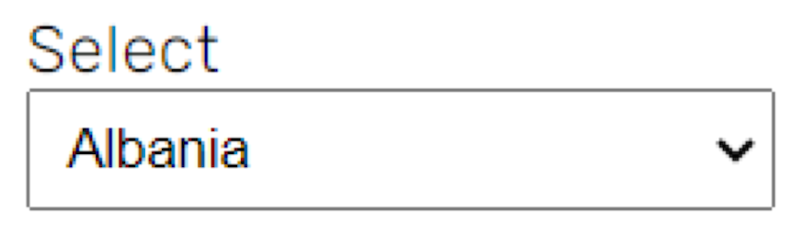
\includegraphics[width=0.9\textwidth]{select/closed.win.chrome.png}
            \caption{\centering Geschlossenes Select Windows Chrome}
            \label{img:closedSelectChrome}
        \end{minipage}
    \end{minipage}
    \hfill
    \begin{minipage}[b]{0.3\textwidth}
        \centering
        \includegraphics[width=\textwidth]{select/opened.win.chrome.png}
        \caption{\centering Offenes Select Windows Chrome}
        \label{img:openedSelectWin}
    \end{minipage}
    \hfill
    \begin{minipage}[b]{0.2\textwidth}
        \centering
        \includegraphics[width=\textwidth]{select/opened.osx.chrome.png}
        \caption{\centering Offenes Select OSX Chrome}
        \label{img:openedSelectOsx}
    \end{minipage}
\end{figure}

Die geöffnete Liste ist bei Firefox als einziges relativ konsistent. 
Sie erscheint in einem grauen Container.
Die anderen Browser sind einstellungsabhängig. 
Sie zeigen den Container weiss oder dunkelgrau (Abbildungen \ref{img:openedSelectWin} und \ref{img:openedSelectOsx}) an. 
Je nach Anzahl der enthaltenen Elemente erscheint die Liste darunter (darüber) oder überdeckt den Container des ausgewählten Wertes. 
Am Wenigsten lässt sich das Element in Safari stylen. 

Da nicht jeder Browser ein Icon anzeigt, ist die Datalist weniger konsistent. 
Safari und Firefox stellen keinen visuellen Hinweis (Abbildungen \ref{img:closedDatalistSafari} und \ref{img:closedDatalistFirefox}) auf die Liste dar.
Safari auf iOS zeigt hingegen in jedem Fall – bezogen auf den textuellen Typ – einen nach unten zeigenden Pfeil an. 
Andere Browser blenden auf der rechten Seite beim Hovern oder beim Besitzen des Fokus das Icon (Dreieck nach unten zeigend) ein. 

\begin{figure}[!htb]
    \centering
    \begin{minipage}[b]{0.25\textwidth}
        \centering
        \begin{minipage}[t]{\textwidth}
            \centering
            \includegraphics[width=0.9\textwidth]{datalist/closed.osx.safari.png}
            \caption{\centering Geschlossene Datalist OSX Safari}
            \label{img:closedDatalistSafari}
        \end{minipage}
        \vspace{0.6cm}\newline
        \begin{minipage}[b]{\textwidth}
            \centering
            \includegraphics[width=0.9\textwidth]{datalist/closed.osx.firefox.png}
            \caption{\centering Geschlossene Datalist OSX Firefox}
            \label{img:closedDatalistFirefox}
        \end{minipage}
    \end{minipage}
    \hfill
    \begin{minipage}[b]{0.37\textwidth}
        \centering
        \includegraphics[width=\textwidth]{datalist/opened.win.chrome.png}
        \caption{\centering Offene Datalist Windows Chrome}
        \label{img:openedDatalistWin}
    \end{minipage}
    \hfill
    \begin{minipage}[b]{0.28\textwidth}
        \centering
        \includegraphics[width=\textwidth]{datalist/opened.osx.chrome.png}
        \caption{\centering Offene Datalist OSX Chrome}
        \label{img:openedDatalistOsx}
    \end{minipage}
\end{figure}

Bei Firefox unterscheidet sich das Öffnen der Liste ebenfalls. 
Wenn das Feld den Fokus noch nicht besitzt, benötigt es zwei Klicks. 
Die anderen Browser lassen die Liste bereits beim ersten Kick erscheinen. 
Die Liste selbst verhält sich je nach Browser und Inhalt verschieden, indem sie seitlich oder darunter (darüber) erscheint. 
Die Übernahme des Dark- bzw. Light-Modes als Container-Farbe hängt vom Browser und dem Anwendungskontext ab.
Die Liste überdeckt das Eingabefeld nie. 
Die Abbildungen \ref{img:openedDatalistWin} und \ref{img:openedDatalistOsx} zeigen Beispiele der geöffneten Datalist. 

Ein Blick auf die mobilen Browser wie iOS-Safari, Android-Firefox und -DuckDuckGo zeigen weitere UI-Unterschiede. 
Für eine bessere Bedienbarkeit zeigen sich die geöffneten Selects auf Android – gegenüber der Desktop-Versionen – in einem anderen Design. 
Die Liste öffnet sich als Dialog-Popup und füllt je nach Anzahl der Werte fast den kompletten Display aus. 
Das selektierte Element besitzt einen ausgefüllten Radio-Button auf der rechten Seite. 
Auf iOS-Browser erhält die ausgewählte Option auf der linken Seite ein Check-Icon (\cmark). 
Der Listen-Container erscheint ähnlich zum OSX-Browser als Dropdown-Liste. 
Nach einer Auswahl schliessen die mobilen Selects automatisch. 

Die Datalist zeigt ihren Inhalt nur bei der Interaktion mit Pfeil auf der rechten Seite. 
Abgesehen von der Grösse der einzelnen Einträge für die Bedienbarkeit unterscheiden sich diese kaum von den Desktop-Versionen.
Die Selektionen erscheinen gegenüber der anderen Optionen in keinem speziellen Design. 

Weitere Inkonsistenzen sind in den Bildern im Anhang \textbf{\ref{chap:existingImgs}} zu sehen. 
Die nachfolgenden Abschnitte \textbf{\ref{sec:edgeBrowser}} bis \textbf{\ref{sec:mobileBrowser}} beschreiben die möglichen Interaktionen. 
Die Tabellen stellen das Datalist, Single- als auch Multiselect einander gegenüber. 
Im Anschluss an die Gegenüberstellungen der Browser weist das Kapitel \textbf{\nameref{sec:summeryExisting}} auf die Inkonsistenzen hin. 


\clearpage
\subsection{Edge Browser}
\label{sec:edgeBrowser}

Die folgende Tabelle \ref{table:interactionEdge} zeigt den Vergleich der typischen Interaktionen in Edge auf Windows. 
Der Vergleich folgt zwischen der Datalist, dem Single- und dem Multiselect. 
Auf Windows verhält sich Edge sehr ähnlich wie Chrome, da die Codebasis beider Browser Chromium ist. 

\import{../tables}{c.edge.tex}


\clearpage
\subsection{Chrome Browser}
\label{sec:chromeBrowser}

Die Gegenüberstellung \ref{table:interactionChrome} beschreibt die Bedienungsmöglichkeiten der existierenden Auswahlkomponenten in Chrome. 
Dabei spielt das System (Windows oder Mac) nur bei der Tastenkombination und nicht bei der Reaktion eine Rolle. 
Auf dem Mac verhält sich Chrome ähnlich wie auf Windows, Designaspekte können sich unterscheiden. 

\import{../tables}{c.chrome.tex}


\clearpage
\subsection{Firefox Browser}
\label{sec:firefoxBrowser}

Die nachfolgende Aufstellung \ref{table:interactionFirefox} zeigt die Reaktionen auf gewisse Benutzerinteraktionen in Firefox. 
Wie auch auf Windows zeigt Firefox auf dem Mac konsistentes Verhalten, jedoch mit typischen OSX Designanpassungen. 
Die Interaktions-Feedbacks auf Mac können sich leicht von der Windows-Version unterscheiden. 

\import{../tables}{c.firefox.tex}


\clearpage
\subsection{Safari Browser}
\label{sec:safariBrowser}

Die Interaktionen auf Safari sind in der Tabelle \ref{table:interactionSafari} einander gegenübergestellt. 
Der Mac Standard-Browser zeigt zu den bisher gesehenen Vergleichen die grösste Abweichung. 

\import{../tables}{c.safari.tex}


\clearpage
\subsection{Browser auf Android \& iOS}
\label{sec:mobileBrowser}

Der Vergleich der Tabellen \ref{table:interactionFirefoxAndroid} und \ref{table:interactionDuckduckAndroid} zeigt, dass auf Android-Geräten Abweichungen existieren. 
Nicht alle Bedienungsmöglichkeiten führen zur selben Reaktion.

\import{../tables}{c.firefox.android.tex}
\import{../tables}{c.duckduck.android.tex}

\clearpage
Im Gegensatz zu den oben gezeigten Andriod-Browser zeigen die meisten iOS-Browser die \codestyle{datalist} und die \codestyle{select}s auf derselben Basis an. 
Der iOS-Safari – als Stellvertreter – zeigt den Vergleich in Tabelle \ref{table:interactionSafariIos} auf. 

\import{../tables}{c.safari.ios.tex}

Wie in den Tabellen \ref{table:interactionFirefoxAndroid} bis \ref{table:interactionSafariIos} zu sehen ist, erlauben Mobilgeräte weniger Interaktionen als Desktop-Computer. 
Zum einen stellen die verschiedenen virtuellen Tastaturen eine geringere Auswahl an Interaktionen an. 
Auf der anderen Seite öffnet sich die virtuelle Tastatur nicht in jeder Situation. 
In Bezug auf die Komponenten Select und Datalist öffnet sich die dynamische Eingabemöglichkeit nur durch das Input der Datalist. 
Dies ist der Grund, wieso in den drei oben dargestellten Tabellen keine Tastatur-Interaktionen bei Selects möglich sind. 
Die Unterschiede bei der Datalist entstehen dadurch, dass nicht jeder mobile Browser die Liste bei Tastatur-Eingaben offen lässt bzw. öffnet. 
Dadurch erklären sich die unterschiedlichen Verhaltensweisen, welche in den Tabellen ersichtlich sind. 

Die Touch-Bedienungen auf der Datalist weisen kaum eine Übereinstimmung auf. 
Das Scrollen als auch das Klicken verhalten sich bei den ausgewählten Mobile-Browsern Safari, Firefox und DuckDuckGo unterschiedlich. 
Das Select zeigt sich in der Interaktion mit dem Finger konsistenter. 


\subsection{Undo / Redo}
\label{sec:undoRedo}

Die Tastatur-Interaktionen Undo\footnote{
    Ctrl \& Z auf Windows; Cmd \& Z auf Mac
} und Redo\footnote{
    Ctrl \& Y auf Windows; Cmd \& Shift \& Z auf Mac
} verhalten sich in allen Desktop-Browsern gleich. 
Beim Select – Single als auch Multi – passiert nichts. 
Im Input-Feld mit der Datalist regieren die Aktionen auf den geschriebenen Text. 
Die einzige Ausnahme ist Safari, welcher das Undo / Redo auf Browserebene ausführt. 
Das bedeutet, die Interaktion betrifft nicht nur das fokussierte Eingabefeld, sondern alle Änderungen im Browser wie das Schliessen von Tabs. 

Von den Mobilgeräten unterstützt nur das iOS-System via Schüttel-Bewegung das Undo bzw. Redo. 
Der iOS-Safari Browser zeigt dieselbe Reaktion wie Safari auf Desktop. 


\clearpage
\subsection{Fazit}
\label{sec:summeryExisting}

Die Gegenüberstellungen der existierenden HTML-Elemente zeigen einige Gemeinsamkeiten, aber auch viele Inkonsistenzen. 
Da die Unterschiede ein Grund für die Entwicklung einer neuen Auswahlkomponente sind, fasst dieser Abschnitt diese nochmals zusammen. 
Im UI existieren über die vier Browser Edge, Firefox, Chrome und Safari als auch den Systemen Mac und Windows teilweise grosse Inkonsistenzen. 
Das System-Theme\footnote{
    Dark- bzw. Light-Mode; auf Systemebene oder Browserebene einstellbar
} spielt für die Darstellung ebenfalls eine grosse Rolle. 
Hierbei spielen das betriebssystemspezifische Styling und die individuellen Implementierungen der Browser eine Rolle. 
Der Fokus dieses Abschnitts liegt auf der Interaktion. 
Das UI ist bereits im Kapitel \textbf{\nameref{sec:uiDifferences}} genauer beschrieben. 

Zwischen Edge und Chrome bestehen keine gravierenden Inkonsistenzen. 
Dies liegt daran, dass die beiden Browser mit der selben Rendering Engine\footnote{
    Mehr dazu steht im Kapitel \textbf{\nameref{sec:browserRenderer}}
} arbeiten. 
Zwischen Mac und Windows bestehen nur die systemspezifischen Unterschiede wie die zu drückenden Tasten (z.B. Home vs. fn \& $\leftarrow$). 

Firefox unterscheidet sich von Chrome in mehreren Interaktionen. 
Während die offene Datalist auf Firefox mit $\leftarrow$ und $\rightarrow$ zwei unterschiedliche Reaktionen zeigt, reagiert sie im Chrome auf dieselbe Weise. 
Das Multiselect zeigt in den beiden Browsern ebenfalls inkonsistentes Verhalten. 
Die Enter-Taste löst auf Firefox im geschlossen Single-Select nichts aus, während Chrome die Liste öffnet. 
Dafür reagiert Firefox im Multiselect auf Tab (Input verlassen), wo Chrome kein Verhalten zeigt. 
Die Interaktionen PageUp/-Down zeigen sich bei Datalist als auch dem Select unterschiedlich. 
Der eine Browser verwendet die View-Höhe als Mass zum Überspringen der Elemente und der andere das \codestyle{size}-Attribut. 
Im geschlossenen Zustand des Single-Select überspringt die Selektion ebenfalls eine unterschiedliche Anzahl Elemente. 
Bei der Interaktion mit der Maus weist das Scrollen auf beiden geöffneten Elementen Inkonsistenzen im Verhalten auf. 

Safari zeigt gegenüber den oben angesprochenen Browsern die grösste Abweichung. 
Einige Aktionen ändern anstelle der Selektion nur das Highlight. 
Zu den Chromium-basierten Browsern - wie Chrome - ist der Apple-Browser am ähnlichsten. 
PageUp/-Down zeigt bei den Einzelauswahl-Elementen ein komplett anderes Verhalten. 
Beim Single-Select ist die Reaktion dieselbe wie beim Drücken von Home/ End. 
Die einzige Interaktion, welche nicht von den anderen Browsern abweicht, ist das Klicken auf ein Element. 

Die inkonsistente Darstellung und Funktionalität dieser Komponenten erschwert eine einheitliche Benutzererfahrung über verschiedene Plattformen hinweg. 
Für eine optimale User-Experience ist die Konsistenzprüfung unabdingbar. 
Diese Erkenntnisse legen den Grundstein für die Entwicklung einer neuen, optimierten Auswahlkomponente. 
Diese soll die bestehenden Probleme adressieren. 
Die bereits erstellte Länderkomponente löst die Inkonsistenzen. 
Details dazu folgen im nächsten Kapitel. 


\section{Länderauswahl Komponente}
\label{sec:countryChoice}

Alternativ zu den bekannten HTML-Elementen \codestyle{datalist} und \codestyle{select} existiert eine weitere, spezielle Auswahlkomponente. 
Die Länderauswahl\citemarktext{
    [\cite{ip5}]
} ist das Resultat des vorausgegangenen Projekts. 
Diese vereinfacht die Selektion eines Landes in einer vorgegebenen Liste. 
Die Komponente ist jedoch nur auf den spezifischen Anwendungsfall – der Wahl eines Landes – getestet. 
Das Design, die Funktionen und die Anwendung unterscheiden sich aber zu den oben genannten HTML-Elementen.


\subsection{Design}
\label{sec:countryChoiceDesign}

Die Länderauswahl erscheint moderner als die alten HTML-Elemente. 
Die Komponente ist in geschlossenem Zustand durch einen immer sichtbaren Container (Abbildung \ref{img:countryInputComponentClose}) visualisiert. 
Darin befindet sich das gewählte Land. 
Ist die Länderauswahl geöffnet, erscheint ergänzend ein Listencontainer mit allen Ländern (Abbildung \ref{img:countryInputComponentOpen}). 
Der Aufbau zeigt sich in einem Spaltendesign – Kontinente links und Länder rechts. 

\begin{figure}[!htb]
    \centering
    \begin{minipage}[b]{0.5\textwidth}
        \centering
        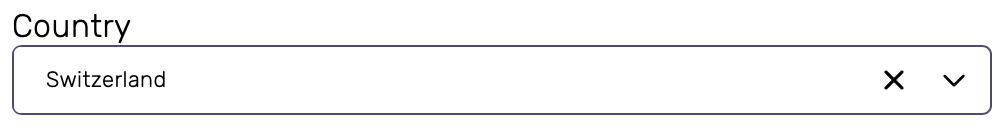
\includegraphics[width=\textwidth]{countryInput-close.png}
        \caption{\centering Geschlossene Länderauswahl}
        \label{img:countryInputComponentClose}
    \end{minipage}
    \hfill
    \begin{minipage}[b]{0.45\textwidth}
        \centering
        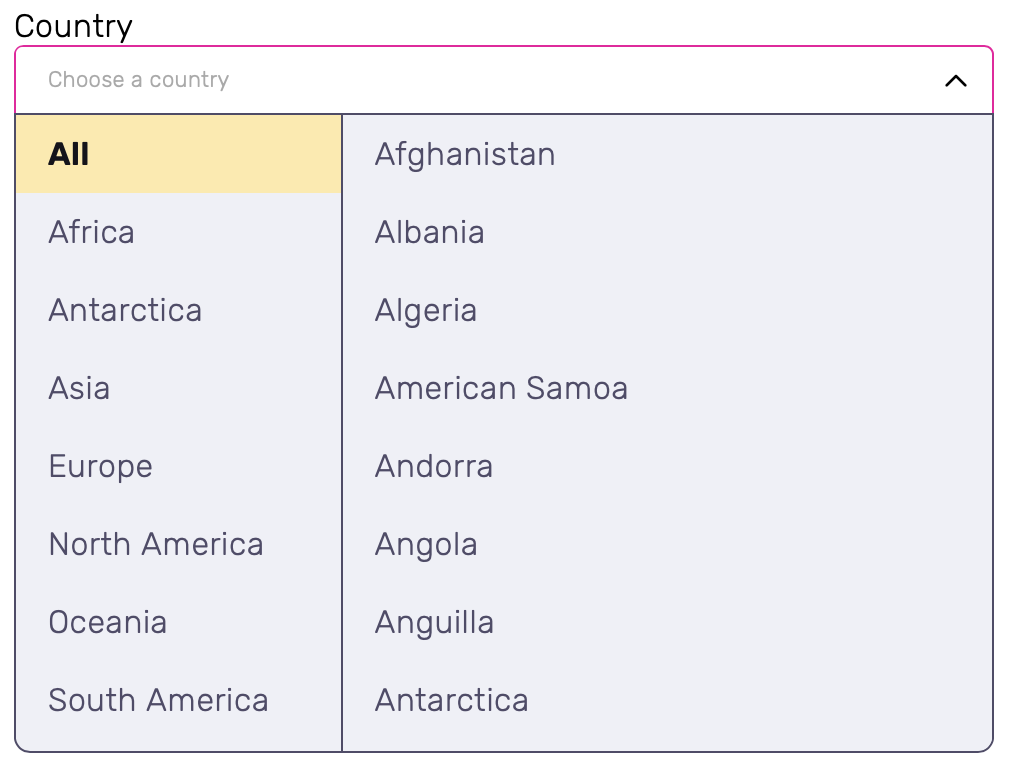
\includegraphics[width=\textwidth]{countryInput-open.png}
        \caption{\centering Offene Länderauswahl}
        \label{img:countryInputComponentOpen}
    \end{minipage}
\end{figure}

Das Design lässt sich einfacher und vielfältiger als bei den Standard HTML-Elementen anpassen. 
Die einzelnen Subkomponenten besitzen Klassen, welche ein einfaches Umstyling ermöglicht. 
Funktionell zeigen sich Übereinstimmungen als auch Unterschiede. 


\subsection{Funktionen \& Interaktionen}
\label{sec:countryChoiceFunction}

Ein grosser Unterschied findet sich in der Funktion des Kontinents. 
Durch die Selektion eines Kontinents reduzieren sich die zur Auswahl stehenden Länder. 
Ist kein spezifischer Kontinent ausgewählt, fällt die Selektion auf \emph{All}. 
Die Komponente besitzt kein integriertes Formular-Feld und benötigt deswegen in dieser Anwendung zusätzlichen Aufwand. 

Die Länderauswahl bietet viele Interaktionen, welche sich bei den HTML-Elementen wiederfinden. 
Die folgende Tabelle \ref{table:interactionCountryInput} zeigt die Interaktionen, welche auf der Komponente implementiert sind. 

\import{../tables}{c.countryInput.tex}

In der Bedienung existieren keine Browser-Inkonsistenzen. 
Die Interaktionen lehnen mehr an denen des Selects als denen der Datalist an. 
Zudem betreffen die Änderungen in der Länder-Spalte nur das Highlight\footnote{
    Die Länderauswahl unterscheidet nicht zwischen Highlight und Cursor Position. 
} und nicht die Selektion. 
Die Selektion benötigt eine Bestätigung mit Enter oder Space. 


\subsection{Anwendung}
\label{sec:countryChoiceUse}

Diese Komponente benötigt in der Anwendung kein HTML. 
Die Einbindung findet via JavaScript statt. 
Der folgende Code \ref{code:countryInputExample} zeigt einen möglichen Anwendungsfall. 

\begin{lstlisting}[style = htmlcssjs, caption = Länderauswahl Beispiel, label = code:countryInputExample]
const container = document.querySelector("#inputContainer");
if (null != container) {
    const countryList = [
        {
            country  : "Austria",
            continent: "Europe",
        },
        /* more country objects */
    ];
    const structureDetail = {
        value      : "",
        placeholder: "Choose a country",
        label      : "Country",
        name       : "country",
    };
    const structureMaster = {
        elementList   : countryList,
        sectionElement: { continent: "All" },
        focusObject   : {},
    };
    const detailController = ChoiceDetailController(structureDetail);
    const masterController = ChoiceMasterController("continent", "country")(structureMaster);
    const view = projectChoiceInput(detailController, masterController, "countryInput");
    container.append(...view);
}
\end{lstlisting}

Wie im Code \ref{code:countryInputExample} ersichtlich sind mehrere Zeilen für die Erstellung der Komponente notwendig. 
Zudem befindet sich die Länderauswahl noch im experimentellen Status. 
Wie das Unterkapitel Future Features aus dem Bericht\citemarktext{
    [\cite{ip5}]
} der Vorarbeit beschreibt, gibt es noch Verbesserungpotezial in der Implementation. 
Da diese Komponente noch nicht lange existiert, ist sie noch in keinem realen Anwendungsfall im Einsatz. 


\section{Anwendungsfälle}
\label{sec:useCases}

Die Standard HTML-Elemente finden in vielen Webapplikationen ihre Anwendung. 
Das bekannteste Beispiel eines Selects ist die Auswahl des Geschlechts. 
Diese Verwendung ist abgesehen vom Design unproblematisch. 
Ein anderer Anwendungsfall ist die Auswahl eines Jahres oder Geburtstags mit drei Selects. 
Das Ausfüllen dieser Situation gestaltet sich schon unangenehmer. 
Dies liegt daran, dass die Suche nach dem gewünschten Wert besonders beim Jahr eher lange dauern kann. 
Besonders mühsam gestaltet sich für Nutzer die Suche nach dem Herkunfts- bzw. Zielland aus einer Liste von ca. 250 weltweit. 
Aber auch den Wohn- oder Destinationsort aus mehreren 100 bis 1'000 (je nach Anwendungsgebiet) auswählen zu müssen, ist sehr zeitaufwendig. 
Die Datalist mit der eingebauten Filterfunktion bietet auf den ersten Blick eine angenehmere Anwendung. 
Das Problem ist jedoch, dass in den meisten Fällen eigene Eingaben unerwünscht sind. 
Als ebenfalls schlechte Alternative bietet sich das Select als Auswahlkomponente an. 
Damit zieht sich die Suche nach einem bestimmten Wert in die Länge – speziell wenn die Optionen nicht in alphabetischer Reihenfolge vorliegen. 
Selbst die Zuhilfenahme der Select-Suche\footnote{
    Durch das Drücken der Anfangsbuchstaben des gesuchten Werte springt die Selektion zur passenden Option
} ist nicht in jeder Situation hilfreich. 
Ein weiteres Anwendungsgebiet findet sich in gewissen Webshop bei den Filter- und Sortierfunktionen wieder. 
Die Komponente zeigt sich unter anderem bei der Auswahl einer Grösse, Farbe oder Kategorie. 
In diesem Beispiel können viele Optionen bzw. Werte ohne klare Reihenfolge in einer Liste auftauchen. 
Dies führt dazu, dass das Auffinden des gewünschten Werts eher schwer fällt. 
All die oben genannten und noch weitere Fälle zeigen verschiedene Probleme auf. 
Die neue Komponente ermöglicht es, die unangenehmen Situationen aufzulösen. 
Mehr Informationen dazu ist im nachfolgenden Kapitel zu lesen. 
